\documentclass[../main/thesis_msc.tex]{subfiles}
\begin{document}
\chapter{Introduction}
\section{Low frequency astronomy}
\begin{tcolorbox}[titlerule=0.5mm,title=\textbf{{\Large History of radio astronomy}}]
$\begin{array}{ll} 
1933 & \textrm{At the Bell Labs, Karl Jansky was trying to understand the source of interference at short }\\ 
     & \textrm{wavelengths in the transatlantic wireless communications, and discovered radiation at 20.5~MHz }\\
     & \textrm{frequency that moved across our sky. He concluded that this radiation was not from Earth.} \\
1937 & \textrm{Grote Weber speculated that these signals were thermal in nature and built a parabolic reflector}\\
     & \textrm{radio telescope with a diameter of 9.5~m and made the first radio map depicting the galactic plane}\\
     & \textrm{and parts of the sky at 160~MHz, and published the paper in 1944  \citep{grote} .}\\
1940s & \textrm{Innovations during the Second World War in the RADAR technology further helped the research.}\\
     & \textrm{J.S. Hey, England and G. C. Southworth discoved that the Sun was radiating radio emission. This}\\
     & \textrm{was followed by discovery of fluctuation in cosmic radiation at radio frequency by  J.S. Hey,}\\
     & \textrm{S.J. Parsons, and J.W. Phillips \citep{fluctuation}. Several discrete radio sources were also}\\
     & \textrm{identified. Radio emission from meteors was also studied.}\\
1950s & \textrm{In the paper \citet{h1}, H. I. Ewen and E. M. Purcell observed the HI 21~cm line from}\\
     & \textrm{radio a Galactic source at declination of 5~deg, as predicted by van de Hulst in 1945. Several}\\
     & \textrm{observatories came to life in this decade such as Cambridge observatory that helped in producing}\\
     & \textrm{the 2C and 3C catalogues. These were the first catalogues to make use of aperture  synthesis}\\
     & \textrm{technique.  Radio emission from Jupiter was also studied at 22~MHz and 3~GHz}\\
     & \textrm{\citep{jupiter}.}\\
1960s & \textrm{A. Penzias and R. Wilson using the Holmdel Horn Antenna at the Bell Labs made one of the most}\\
     & \textrm{important astrophysical discoveries: the Cosmic Microwave Background, for which they were}\\
     & \textrm{awarded the Nobel prize in 1978. This decade also marked the discovery of pulsars by J. Bell}\\
     & \textrm{in her article "Little Green Men, White Dwarfs or Pulsars?" \citep{jocelyn}. A. Hewish }\\
     & \textrm{received the Nobel prize in 1974 for this discovery.}\\
1970s & \textrm{Hulse and Taylor discovered the first binary pulsar system at Arecibo, and thus proved the}\\
     & \textrm{presence of Gravitational wave radiation, after conducting pulsar timing for nearly 20 years}\\
     & \textrm{\citep{binary}. They were awarded the Nobel prize for this discovery in 1993.}\\
     & \textrm{The first global radio telescope was formed in 1976 to observe water maser sources.}\\
1980s & \textrm{The need for better resolution gave rise to the construction of interferometers such as TPT}\\
     & \textrm{in Clark Lake, observing at the frequency of 57.5~MHz. The first self calibration for VLA}\\
     &\textrm{images was done. Astronomical Image Processing Software (AIPS) was also released. }\\
1990s & \textrm{VLA system observing at 74~MHz frequency was used. Planck black-body spectrum for the CMB}\\
     & \textrm{was measured, and the anisotropy was discovered for the first time using COBE satellite}\\
     & \textrm{\citep{cobe}. Mather and G. Smoot were awarded the Nobel prize for this discovery in 2006.}
\end{array}$
\end{tcolorbox}
During 1970 to 2000, due to the need for higher resolutions, studies were mostly focused on radio frequencies of $>$ 1~GHz (see section \ref{sec:resolu}. Several telescopes sensitive to the higher radio frequency were made- VLA, ATCA, GMRT, MERLIN and single dish telescopes such as Effelsberg, Arecibo and Lovell. Interest in low frequency radio astronomy began when many sources were seen to have inverted spectra due to synchrotron self-absorption or free-free absorption (see section \ref{sec:process}). NRAO and the Naval Research Laboratory completed the implementation of VLA at 73.8~MHz in 1998 and found that ionospheric phase shifts posed the biggest difficulty in calibrating data. It was found that self-calibration could help with this \citep{74MHz}. In the paper \citet{vlss}, 70,000 sources were cataloged  at 77~MHz, including several extra-galactic sources such as high redshift galaxies, galaxy clusters, Supernova Remnants (SNRs) and Galactic sources such as pulsars. It covers almost  95\% of the 3$\pi$~sr of sky above -30~deg declination. This survey is very useful for calibration in LOFAR and has been revised to give 95,000 sources in \citet{vlss2}. In the paper \citet{ska}, a 1~km$^2$ array was proposed so as to study the neutral hydrogen at cosmological distances, called the Square Kilometer Array (SKA). Due to cost constraints, the concept of Phased Arrays \citep{lof1} using dipole antennae was proposed, which then gave rise to LOFAR.

\section{LOw Frequency ARray- LOFAR}    
LOFAR or LOw Frequency Array is a radio interferometer mainly located in the Netherlands. It consists of two types of receiving elements: the Low Band Antennae (LBA) that covers the frequency range of 10-90~MHz, and the High Band Antennae (HBA) that covers the frequency range from 110-250~MHz. It is interesting to note that the pointing in LOFAR is done by applying digital delays to elements of individual stations. The LBA (shown in Figure \ref{lba}) in reality can only operate between the frequency range of 30-80~MHz due to the presence of Radio Frequency Interference (RFI) at the lower frequency regime and the commercial FM band at the higher regime. An LBA dipole can detect two orthogonal linear polarizations, with an all-sky sensitivity. The dipoles themselves make up the elements to do beam-forming. The HBA (shown in Figure \ref{hba}) can reach frequency only upto 240~MHz due to RFI. 16 antennae are grouped under one ``tile", and each of these tiles can form a ``tile beam". Each tile does the beam-forming with the help of an analogue beam-former that adds a delay to each dipole.
\begin{figure}%
    \centering
    \subfloat[]{{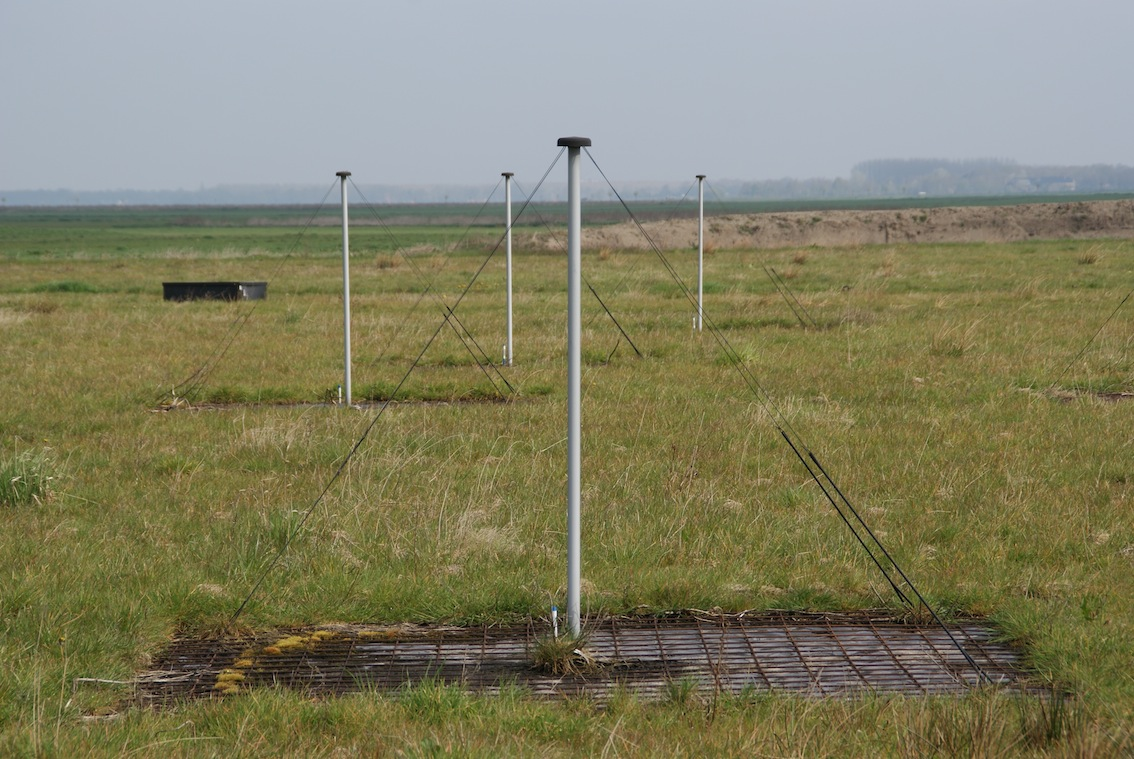
\includegraphics[width=6.5cm]{lba.png} }%
    \label{lba}}
    \qquad
    \subfloat[]{{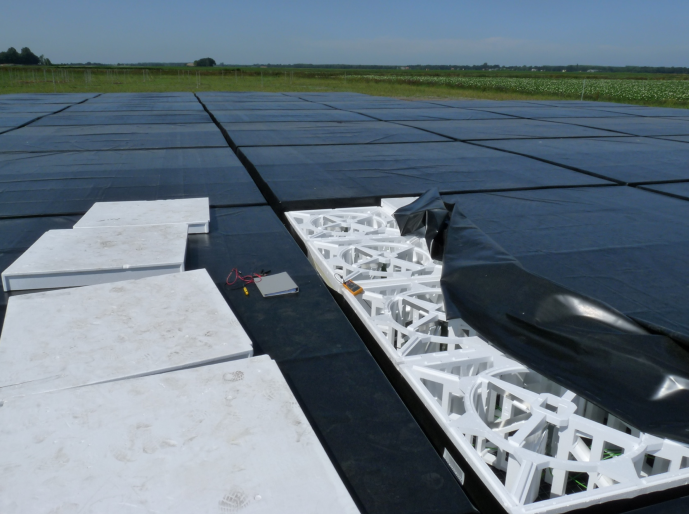
\includegraphics[width=5.8cm]{hba.png} }
    \label{hba}}%
    \caption{The different Antenna types in LOFAR. \textit{Left:} Low Band Antenna is held upright by the two copper wires connected to its top that help in detection of the two polarizations, and the ground mesh \citep{lba}. \textit{Right:} Each High Band Antenna tile has 16 aluminium elements held together by an expanded polystyrene structure \citep{LOFAR}}%
\end{figure}
LOFAR has a dense core i.e., it has numerous short baselines that are very helpful in the study of diffuse emission. It currently has 24 core stations (CSs) located in Exloo, Netherlands, and 14 remote stations (RSs) located all over the Netherlands. These stations have 96 LBAs and 48 HBAs with 48 digital Receiver Units (RCUs). These arrangements can be seen the Figure \ref{lofar_arrangement}. The international stations (ISs) are present in Germany (5 stations), Great Britain (1 station), France (1 station), Sweden (1 station) and Ireland (1 station). A summary of the arrangement and other properties of LOFAR are given in Table \ref{lofar_specs}. 
\begin{table}[t]
        \centering
        \begin{tabular}{ccc}
            \toprule
            \textbf{Characteristic} & \textbf{Value} & \textbf{Comments} \\ \midrule
            Frequency range & 10-90~MHz & LBA \\
                                        & 110-190~MHz & HBA \\ \\
            Shortest baseline & 68~m & among CSs, RSs and ISs (unprojected values) \\ \\
            Maximum baseline & 3.5~km & CSs \\
                                         & 121~km & RSs \\
                                         & 1158~km & ISs \\ \\
            Number of Polarizations & 2 & \\ \\
            Bandwidth & 48~MHz & 16-bit mode \\
                          & 96~MHz & 8-bit mode \\ \\
            Maximum number of & 244 & 16-bit mode\\
            simultaneous beams & 488 & 8-bit mode\\
            \bottomrule
        \end{tabular}
        \caption{LOFAR specifications, all obtained from \citep{LOFAR}}
        \label{lofar_specs}
    \end{table}
    
\begin{figure}
        %\centering
        \subfloat[]{{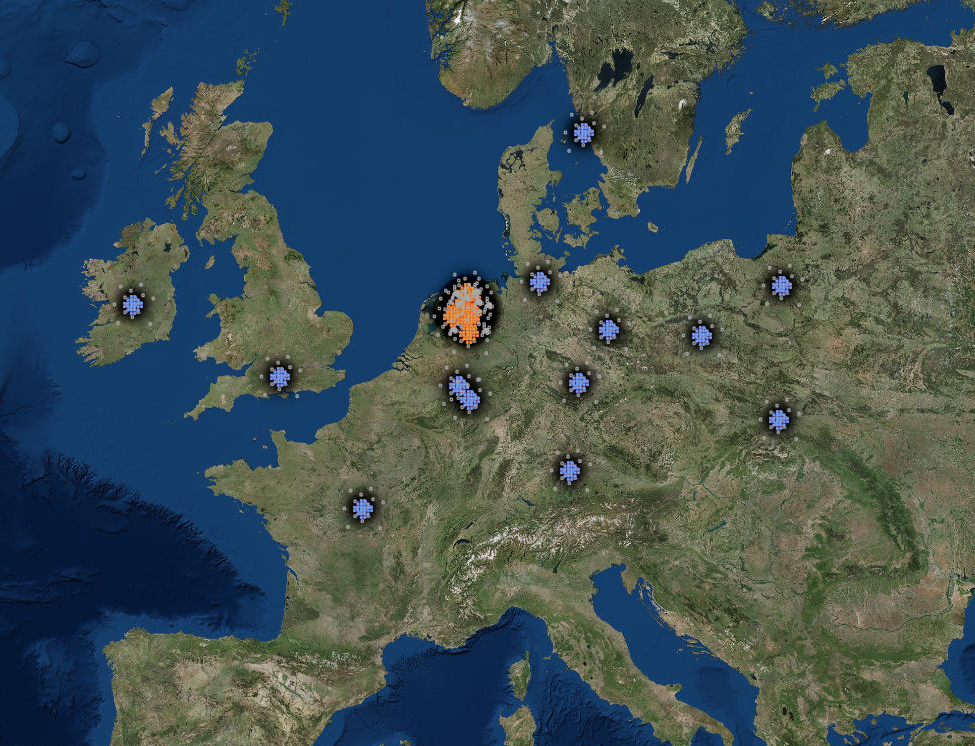
\includegraphics[width=6cm, height=5cm]{lofar_arrangement.png}}}
        \centering
        \subfloat[]{{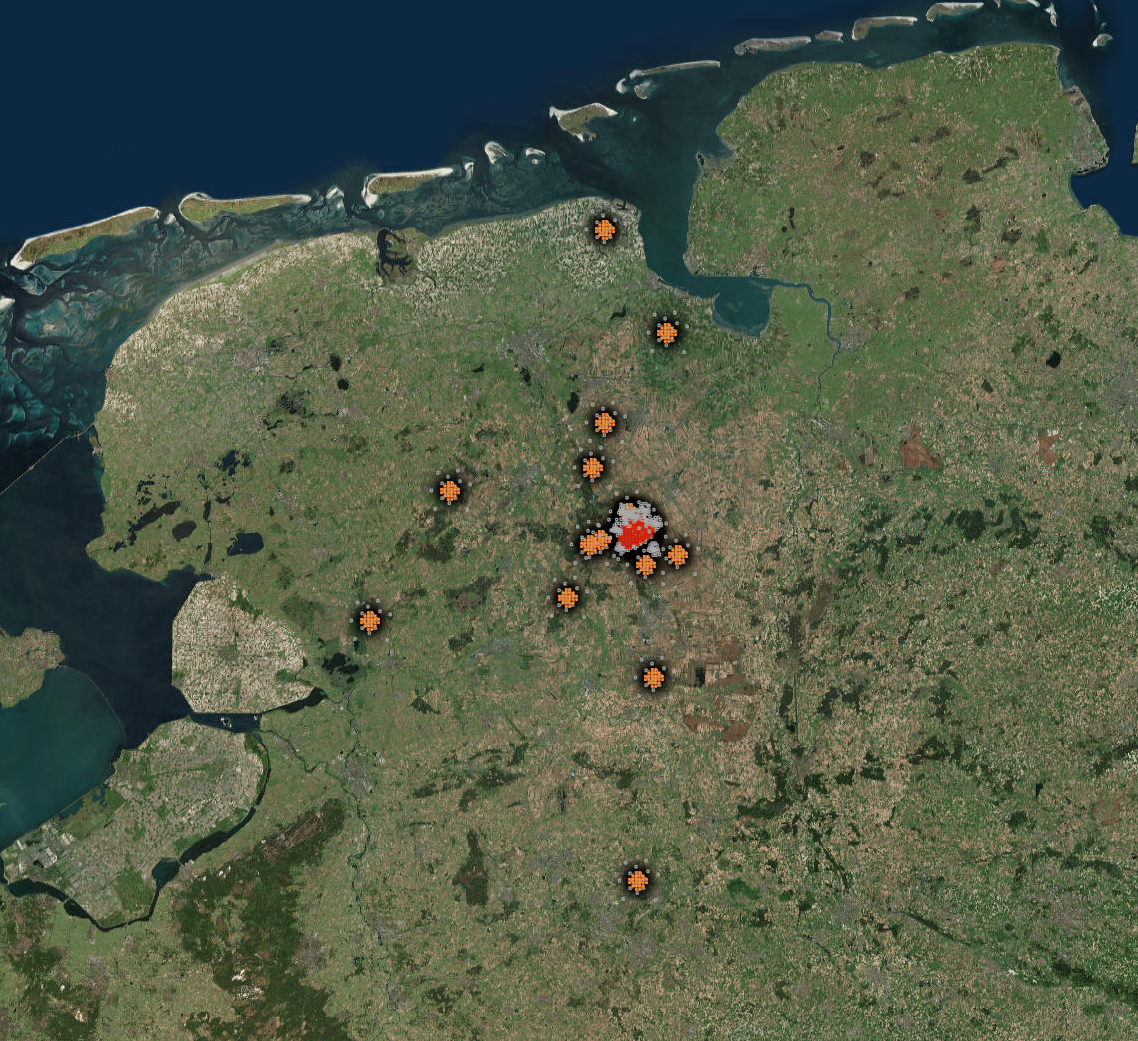
\includegraphics[width=6cm, height=5cm]{lofar_arrangement_core.png}}}
        \caption{Arrangement of the LOFAR stations in Europe. \textit{Left:} The blue regions represent the international stations. The orange regions in the represent the remote stations. \textit{Right:} On a closer look, the red regions represent the core stations. These images were obtained from \url{http://astron.nl/lofartools/lofarmap.html}}
        \label{lofar_arrangement}
        \end{figure}
The data from both LBA and HBAs are sent to the receiver unit (RCU), where digitization using Analog to Digital converter through coaxial cables. Then the beam-forming is done in the digital electronics section. After that, the signal is either sent to the Cobalt correlator in Groningen or recorded and dealt with locally based on the observing mode. LOFAR has three main observing modes that are explained in the Table \ref{moooo}. 
\begin{table}
\centering
\begin{tabular}{cc}
\toprule
\textbf{Modes} & \textbf{Description}\\ 
\midrule
Interferometric & Gives visibility data to be used in surveys and for single souce imaging. \\
Beam Formed & This is used when high time resolution is needed e.g., for pulsars, cosmic rays, etc. \\
Direct Storage & Uncorrelated data is recorded locally for single station all sky imaging\\ & or local Transient Buffer Board (TBB) experiments.\\
\bottomrule
\end{tabular}
\caption{The LOFAR imaging modes}
\label{moooo}
\end{table}
The data streams from the individual dipole antennae are sent to the Central Processing (CEP) facility located in Groningen through a dedicated network high speed fibers. The data is then processed in the Blue Gene/P supercomputer. During this processing, the signal from the stations is correlated, and the beam-forming is done. After this, the data is given to the storage cluster. The data is processed using several reduction pipelines before being stored in the LOFAR long term archive (LTA) for scientific purposes. 
The CEP4 cluster, part of the LOFAR clusters, is used to do the initial processing and calibration using pipelines on the data from the Cobalt correlator (in Groningen). Another cluster- CEP3, used by LOFAR users to decide the strategy to be used for calibration. Once the data has been processed, it is made available on Long Term Archive (LTA).\\
\noindent Some of the packages used for the calibration of LOFAR data are: Astronomical Image Processing Software(AIPS), Common Astronomy Software Applications \citep[CASA ;][]{casa}, AOFlagger (helps in flagging RFI) \citep{aoflagger}, SAGECal (calibration package), dysco (compressing storage manager for measurement sets) and several others, which will be visited upon during the course of the thesis.
Some of the performance metrics of LOFAR are described below:
\begin{itemize}
\item The rate of change of the ionospheric phase above the Netherlands is 1~rad per 15~s in the 110 to 190~MHz band \citep{LOFAR}. For LBA, water may affect the gain by the order of 10\%,  though HBA amplitudes remain pretty stable. These effects of ionospheric phase shift can be significantly depreciated using the method of self-calibration. 
\item The angular resolution is from 0.5~$\deg$  to sub-arcsec levels, depending on the declination of the source, and the array configuration.
\item One the factors that affect the image quality is the uv coverage. As can be seen from theFigure\ref{uv}, we can easily see that LOFAR has a very dense core and there are several long baselines, for better resolution.
\begin{figure}
\centering
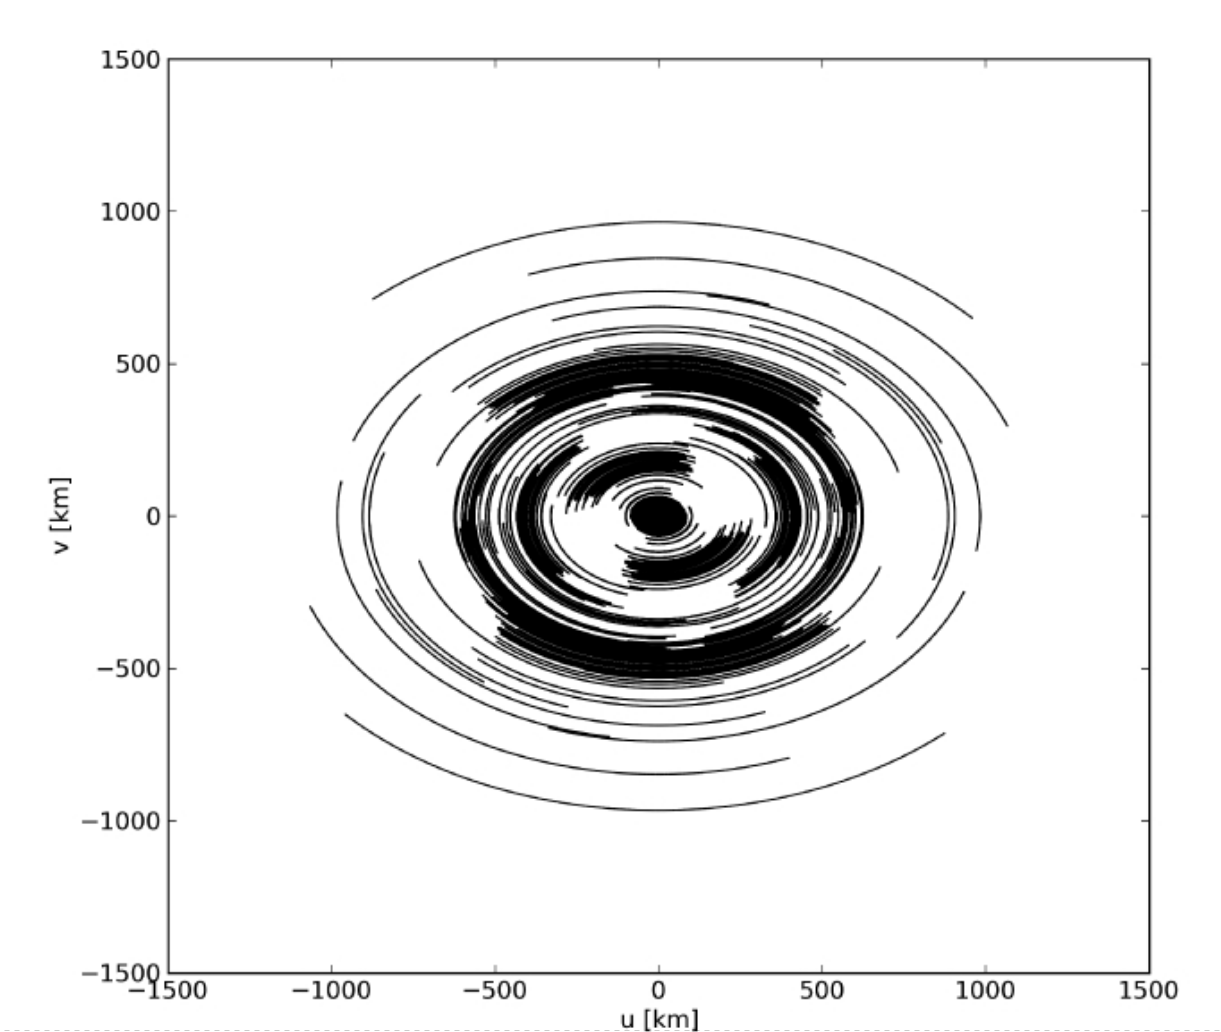
\includegraphics[scale = 0.2]{uvcoverage.png}
\caption{The uv coverage of LOFAR including all core, remote and international stations \citep{LOFAR}. The simulation of this uv-coverage is based on a hypothetical 6 hour observation of a source at a declination of 48~$\deg$ between 30-78~MHz using single beam with bandwidth of 48~MHz.}
\label{uv}
\end{figure}
\item The band-pass of LOFAR is affected by several factors: the station beam- which is in itself frequency dependent, the interaction between the antenna elements and the low noise amplifier (LNA). Inorder to take care of this, a digital correction is applied within each 0.2~MHz subband.
\item The Field of View (FoV) of LOFAR ranges from 2 to 1200~$\deg ^2$, and is given by:
\begin{equation}
\textrm{FoV}=\pi\left(\frac{\textrm{FWHM}}{2}\right)^2.
\end{equation}
\end{itemize}
\section{Importance of low frequency astronomy (LOFAR Key Science Projects)}
LOFAR covers frequencies from 10~MHz to 250~MHz. As can be seen from Spectral Energy Distribution (SED) plot in the Figure \ref{sed}, the radiation in this regime is from non-thermal synchrotron emission\footnote{We will visit this in section \ref{sec:sync}.}, for a star burst galaxy\footnote{This is somewhat different for other astrophysical soures (see \citet{2001isra.book.....T}, Figure 1.1)}. Furthermore, the flux density of synchrotron radiation increases at lower frequencies (until effects such as synchrotron self absorption and ionization loses take over and reduce the synchrotron flux density) and hence, it gets easier to study the radiation from these low energy cosmic ray electrons. It is also interesting to note that low frequency radiation is produced by low energy electrons that have not been affected much energy loss. This includes the older electrons that have traveled farther from their point of origin, such as SNRs\footnote{Low energy electrons are also present at the point of origin, while high energy electrons are \textit{only} present close to their injection sites.)}. Therefore, they can help us study galactic disks and the halos of galaxies. In this section, the different Key Science Projects (KSPs) undertaken by the LOFAR community are explained.
\begin{figure}
\centering
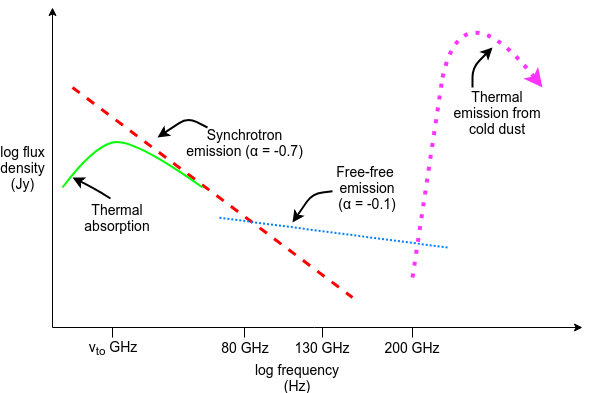
\includegraphics[scale = 0.65]{SED_corr_freq.png}
\caption{This is the Spectral Energy Distribution plot, showing the processes that are dominant at various frequency ranges. Thermal emision from cold dust dominates the spectrum for infrared frequencies ($>$200~GHz). For frequencies between 80 to 200~GHz, free-free emission dominates the spectrum. From frequencies below 80~GHz, synchrotron emission dominates the spectrum. In regions where the total opacity of the region becomes $\approx$ 1 or more, the turn over is seen, and thermal absorption lowers the synchrotron flux density. This plot is only representation to show of various processes for a star forming galaxy, and cannot be taken as an accurate depiction1q of the frequency ranges indicated. This is because these process differ for varying objects, such as in compact sources such as AGNs, synchrotron self-absorption may be responsible for the turn over seen at low frequencies, and not thermal absorption. Also, for high redshift galaxies, these frequency ranges are different.}
\label{sed}
\end{figure}
\paragraph{Epoch of Reioniation KSP:} According to the $\Lambda$CDM model, there existed a stage 400,000 years after the Big Bang, when the Universe became transparent leaving only a relic radiation which we now call the Cosmic Microwave Background radiation. This era came to be known as the ``Dark ages", and happened when the ions and electron combined. It came to an end 400 million years later, when objects such as stars and Black Holes were formed, and assembled into proton-galaxies. This era came to be known as the ``Epoch of Reionization", or ``Cosmic dawn". Several questions still need to be answered about the formation of the Universe, such as what resulted in the end of the Dark Ages, and what gave rise to the EoR, and how are Black holes formed? One of the best ways to understand and answer these questions is by studying red-shifted HI 21~cm emission line using LOFAR core elements.
\begin{figure}
\centering
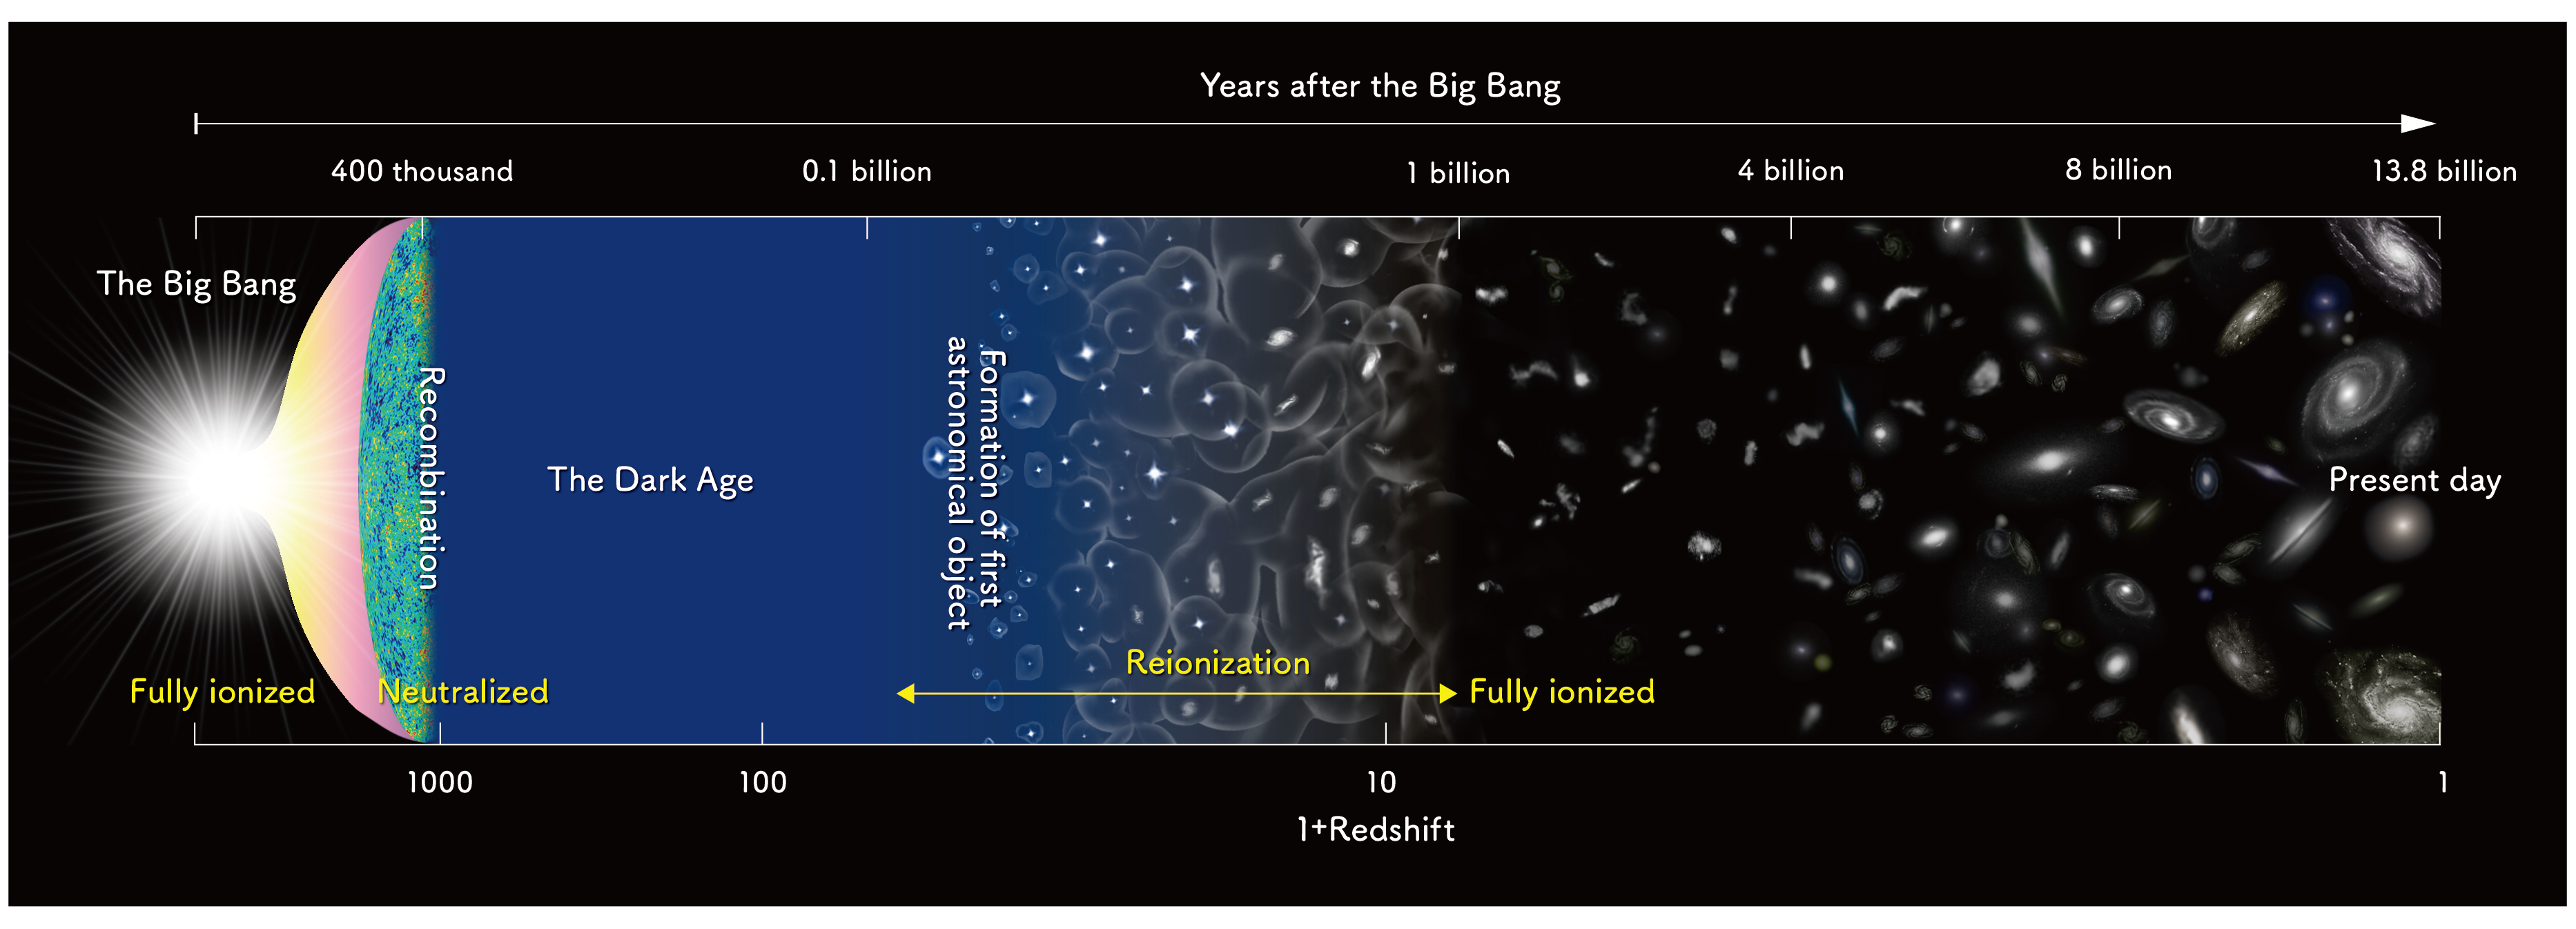
\includegraphics[scale = 0.5]{eor.jpg}
\caption{This is a schematic diagram depicting the lifetime of our Universe. At redshift z $\approx$ 1100, the dark ages begin, and EoR begin at z $\approx$ 6 -- 12. Courtesy of National Astronomical Observatory of Japan (NAOJ).}
\end{figure}
\paragraph{Surveys KSP:} LOFAR can be used for large sky surveys owing to its large instantaneous field of view. These surveys can help us study high red-shifted galaxies (which will help us understand the formation and evolution of massive galaxies), clusters of galaxies (which will help us understand the characteristics of magnetic fields and CR acceleration) and cosmic star formation history of Universe.
\paragraph{Transients KSP:} This entails the study of transients such as pulsars, Gamma-Ray Bursts, X-ray binaries, radio supernovae and flare stars. Due to LOFAR's wide field and good sensitivity, it would help us do extensive time-domain studies, and discover new transient events.
\paragraph{Cosmic Rays KSP:} The Cosmic Ray (CR) flux follows the simple power law: $\frac{dN}{dE} \propto E^{-\gamma}$. Hence, for energies above 10$^{19}$eV, only one particle per century per square kilometer reaches Earth. Hence, large effective areas are required to do proper statistics. At the energy of $\sim 5 \times 10^{15}$, $\gamma$ changes from 2.7 to 3.1 in the CR spectrum, and is called the ``knee" of the spectrum. After this ``knee", the composition of the CRs is not well known. This knowledge can be obtained with the help of LOFAR, which will help us understand the acceleration and propagation mechanisms, andFigureout the universal acceleration process. One of the candidates for the acceleration process is the diffusive shocks in the radio lobes of radio galaxies. Furthermore, extensive research on air showers at ground level, can help us study new particle physics.
\paragraph{Solar KSP:} Sun is an intense source of radio thermal emission, and gives rise to solar flares and Coronal Mass Ejections (CMEs) which can be studied with the help of LOFAR. Sun also has an effect on the space environments, and communication technology on earth, and hence, this project mainly aims to study the space weather and solar physics.
\paragraph{Cosmic Magnetism KSP:} Magnetic fields are very important to understand the Universe. LOFAR, due to its wide bandwidth can help us do best precision studies of Faraday rotation and weak magnetic fields. With the help of Faraday tomography/ Rotation Measure (RM) Synthesis can help us obtain polarized radio synchrotron emission. 
\subsection{Astrophysical processes at Low Frequencies}
\label{sec:process}
At low frequencies, several astrophysical process are important. In the Figure \ref{sed}, one can see the various process that become important at different frequency ranges. In the lower frequencies from around 10~GHz to 10~MHz, synchrotron emission is the dominant process. This process was first explained by a German astronomer named Karl-Otto Kiepenheuer in the year 1953. As the wavelength increases, the flux density of synchrotron emission increases. This helps us detect even the lowest intensity emission from the cosmic ray electrons. In this section, the numerous emission and absorption astrophysical processes that need to be taken into account whilst trying to explain the resultant emission at the frequencies that LOFAR detects are explained. 
\paragraph{Synchrotron emission:}
\label{sec:sync}
When charged particles (mostly electrons) move around magnetic field lines at relativistic speeds, they emit photons. This emission of photons is called synchrotron emission and is non-thermal, as these relativistic electrons have a power law energy distributions:
\begin{equation}
\textrm{N(E) dE = E}^{-p} \textrm{dE}
\end{equation}
\noindent Here, N(E) dE is the number of electrons per unit volume in energy interval E and E + dE, and `\textit{p}' is the electron spectral index.
\noindent Let us consider a single electron (since synchrotron emission mostly comes from accelarating electrons), moving with velocity {\textbf{\textit{v}}} in a magnetic field {\textbf{\textit{B}}}. The electron energy is given by E = $\gamma$ mc$^2$, where $\gamma$ is the Lorentz factor and c is speed of light, and m is mass of electron. Its motion can be described by:
\begin{equation}
\frac{\textrm{d}}{\textrm{dt}} (\gamma \textrm{m}  {\textbf{\textit{v}}} ) = \frac{\textrm{e}}{\textrm{c}} (  {\textbf{\textit{v}}} \times  {\textbf{\textit{B}}} )
\end{equation}
\noindent If we resolve {\textbf{\textit{v}}} into components parallel and perpendicular to the magnetic field represented as  {\textbf{\textit{v$_{\|}$}}} and {\textbf{\textit{v$_{\bot}$}}}, then {\textbf{\textit{v$_{\|}$}}} remains constant with request to time, and $\frac{ \textrm{d{\textbf{\textit{v$_{\bot}$}}}}}{dt}$ = $\frac{\textrm{e}}{ \gamma \textrm{mc} }$ ({\textbf{\textit{v$_{\bot}$}}}$\times${\textbf{\textit{B}}})
\noindent The electron thus moves in a helical path centered at the magnetic field lines. The pitch angle, $\theta$, of the trajectory of electron can be easily obtained from the velocity components. The angular gyro-frequency is given by the equation:
\begin{equation}
\omega_g = \frac{\textrm{e}{\textbf{\textit{B}}}}{\gamma \textrm{m}}
\end{equation}
\noindent From theFigure\ref{sync}, we can see that the electron will radiate in the Lorentz transformed beam pattern, and the forward power is in the beam of the angle $\frac{2}{\gamma}$.  
\begin{figure}
\centering
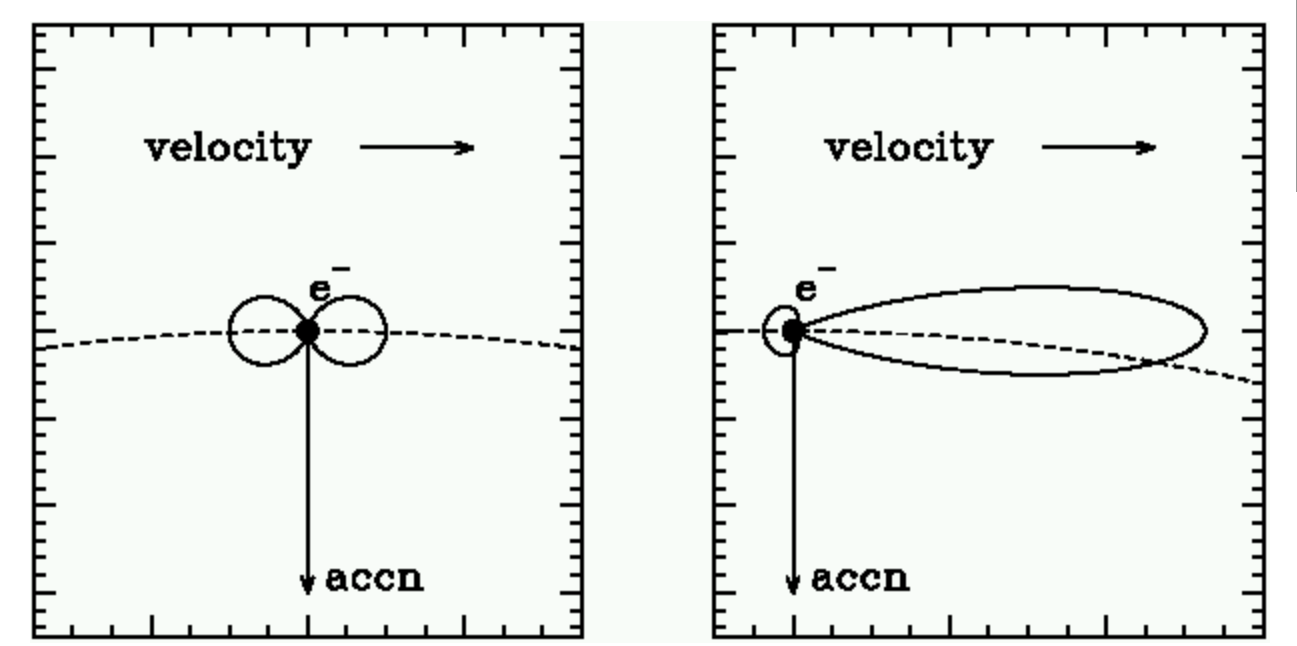
\includegraphics[scale = 0.2]{sync.png}
\caption{When an electron moves at relativistic speeds, the sin$^2$ radiation pattern is Lorentz transformed. \textit{Left:} The radiation pattern of a non-relativistic electron. \textit{Right:} The relativistic radiation pattern. This image has been taken from \url{http://www.astro.utu.fi/~cflynn/astroII/l4.html}}
\label{sync}
\end{figure}
\noindent The full derivation of the emission spectrum for a single electron can be seen in \citet{longair}. Here, I have merely written down the final equation. $I_{\|}$ and $I_{\bot}$ represent the the polarizations of the emission and $T_r$ represents the period of the electron in orbit.
\begin{equation}
j(\omega) = \frac{I_{\|} + I_{\bot}}{T_r} = \frac{\sqrt{3} e^3 \textbf{\textit{B}} sin \theta }{8 \pi^2 \epsilon_0 \text{cm}}
\end{equation}
Here, $F(x) = x \int_x ^{ \infty } K_{\frac{5}{3}} (z) dz$ where $K_{\frac{5}{3}}$  is the modified Bessel function of the order $\frac{5}{3}$ and $x= \frac{2\omega a }{3c \gamma^3}.$ c is the speed of light and m is the mass of the particle.
From this equation, one may find the emission from a population of electrons which is seen in synchrotron emission. For the distribution of electron described earlier, the total emission for electrons with a constant pitch angle can be given by:
\begin{equation}
J(\omega) \propto \kappa \textbf{\textit{B}}^{\frac{(p+1)}{2}} \omega^{-\frac{(p-1)}{2}}
\end{equation}
Hence, the spectral index of synchrotron emission is represented as $\alpha$ and is equal to the power on the omega function.
\paragraph{Free-free emission:}
Another process that is important at lower frequencies, is the free-free emission. Deceleration of electrons due to the presence of a charged particle results in thermal emission\footnote{Thermal emission is produced by a source whose emitting particles are in local thermodynamic equilibrium (LTE).}, which is termed as free-free emission or Bremsstrahlung (from the German words `bremsen' - to brake and `strahlung'  - radiation). The energy/frequency of the proton depends upon the loss in kinetic energy of the particle (h$\nu$ = E - E'). This process usually is seen in an ionized gas mediums, such as an H II region. It results in the steepening of the spectra, however, at such long wavelengths, its effects are severely diminished due to the presence of the steep synchrotron spectrum.
\paragraph{Absorption processes:}
For every emission process, there should exist an absorption process, according to the Principle of Detailed balance. These absorption processes usually take place in the star forming regions, while the regions with less electron density have a steeper spectra and are not affected by these effects.
\begin{itemize}
\item \textit{Synchrotron self-absorption} The brightness temperature of a particle in Local Thermodynamic Equilibrium (LTE) cannot exceed its kinetic temperature. If a synchrotron source has a Maxwillian energy distribution (in LTE), then the synchrotron self-absorption prevents the particles from attaining the brightness temperature greater than the particle temperature.
\item \textit{Free-free absorption} If an electron absorbes a photon when moving near an ion, it is called free-free or thermal absorption. This absorption usually takes place in H\,II regions which are in Local Thermodynamic Equilibrium. \\
One could use Kirchhoff's law to obtain the absorption co-efficient, which is given by:
\begin{equation}
\kappa_{\nu} = \frac{\epsilon_{\nu}}{\textrm{B}_{\nu}\textrm{(T)}} = \frac{\epsilon_{\nu} \textrm{c}^2}{2\textrm{kT}\nu^2}
\end{equation}
Here, $\epsilon_{\nu}$ is the emission co-efficient, k is Boltzmann constant. T is the temperature of the H\,II region and c is the speed of light. 
\begin{equation}
\epsilon_{\nu} \propto \textrm{ln}\left(\frac{\text{A}}{\nu}\right)
\end{equation}
where A=$\frac{\textrm{m}_e}{2\pi\textrm{Ze}^2}$ (after several approximations). m$_e$ and Ze is the mass of electron and the charge of the ion respectively. \\ \\
Hence, one can use the numerical approximation of $\kappa_{\nu} \propto \nu^{-2.1}$ to understand the dependence of frequency on the absorption coefficient. The total opacity, $\tau_{\nu}$ is the integral of the coefficient of absorption along the line of sight (los):
\begin{equation}
\tau_{\nu} = \int_{\textrm{los}}-\kappa_{\nu} \textrm{ds}
\end{equation}
The flux density of the source is given by:
\begin{equation}
\textrm{S}_{\nu} \propto \frac{2\textrm{kT}\nu^2}{\textrm{c}}\tau_{\nu}
\end{equation}

At very high frequencies, the opacity $\tau_{\nu} << $ 1, and the H\,II regions are almost transparent. However, as the frequency becomes lower, the total opacity increases. The region becomes opaque and its spectrum approaches that of a black body, as can be seen in the Figure \ref{h2re}. 
\begin{figure}
\centering
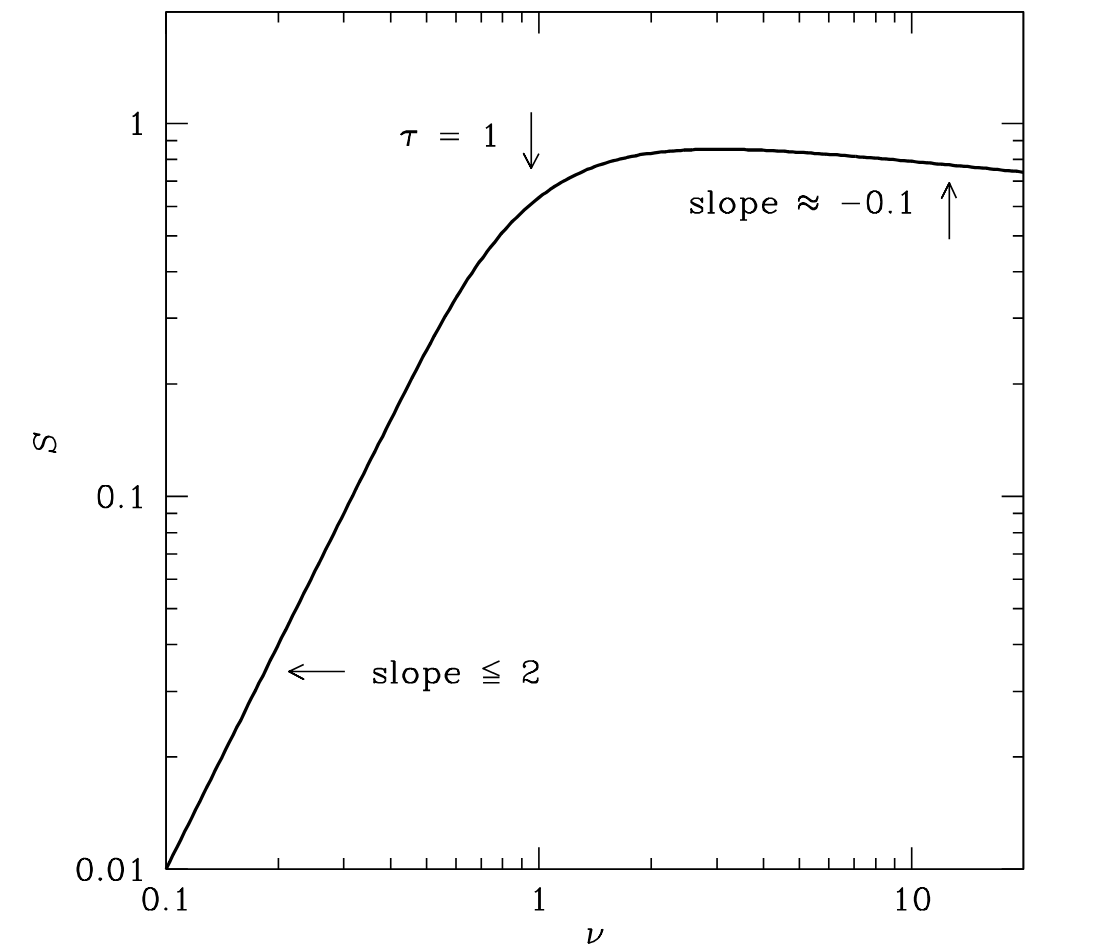
\includegraphics[scale = 0.18]{h2region.png}
\caption{The radio spectrum of an ideal H\,II region. Here, thermal emission and absorption process are dominant, because an H\,II region is in LTE. At low frequencies, the slope is 2.0, while the slope at higher frequencies is around -0.1. At the total opacity of around 1, the turn over occurs. This is when free-free absorption is seen to dominate. This image has been taken from \url{https://www.cv.nrao.edu/course/astr534/FreeFreeEmission.html}.}
\label{h2re}
\end{figure}
When the total opacity $\tau_{\nu} \approx$ 1, the slope is seen to have the turn over (it changes from $-$0.1 to +2). Thermal absorption thus results in the flattening of the spectrum of a galaxy at extremely low frequencies. Thermal absorption thus results in flattening of the spectrum of a galaxy with high star formation rate, the total opacity approaches the value of 1 at much higher frequencies than galaxies with low star formation. A numerically feasible equation to obtain the total opacity is given by the Equation \ref{tau}. 
\begin{equation}
\tau_{\nu} \approx 3.28 \times 10^{-7} \left(\frac{\textrm{T}_e}{10^4}\right)^{-1.35}\left(\frac{\nu}{\textrm{GHz}}\right)^{-2.1}\left(\frac{\textrm{EM}}{\textrm{pc/cm}^{-6}}\right)
\label{tau}
\end{equation}
Here, EM is the emission measure which is integral of the square number density of electrons along the los, and is given by the Equation \ref{EMea}. Here N$_{\text{e}}$ is the electron number density. 
\begin{equation}
\text{EM} = \int_{\text{los}} \left(\frac{\text{N}_{\text{e}}^2}{\text{cm}^{-3}} \right) \text{d}\left(\frac{\text{s}}{\text{pc}}\right)
\label{EMea}
\end{equation}
With the help of turn-over frequency, i.e., the frequency at which the slope of the power spectrum in the H\,II region changes to 2 and optical depth $\tau_{\nu}$ is 1, one may be able to obtain the value of EM, and thus obtain the electron density present along the line of sight. $\nu_{\text{to}}$ in the Equation \ref{to} is the turn over frequency.
\begin{equation}
\text{EM}=3.048\times10^{6} \left(\frac{\textrm{T}_e}{10^4}\right)^{1.35}\left(\frac{\nu_{\text{to}}}{\textrm{GHz}}\right)^{2.1}
\label{to}
\end{equation}


\end{itemize}
\paragraph{Loss processes}
Emitting cosmic ray electrons lose their energies in several ways, some of which are listed below:
\begin{itemize}
\item \textit{Ionization loss} When a cosmic ray electron strikes a neutral particle, it may impart some of its energy to it, which may result in ionization, giving rise to an ion. These losses are seen in the nuclear regions of star burst galaxies, and result in the flattening of the spectral index.
\item \textit{Inverse Compton loss} When a cosmic ray electron with sufficiently high energy encounters a photon, its energy may be used to increase the energy of the photon. This may result in a photon going from X-ray regime to Gamma regime. 
\item \textit{Adiabatic loss} Ultra relativistic particles e.g. in SNRs, may lose their internal energy during expansion and result in the dimming of synchrotron emission. This loss mechanism is termed as adiabatic.
\item \textit{Free- free loss} When a cosmic ray electron is decelarated in the presence of an ion, it loses some of its energy in form of a photon. The energy of the photon comes from the kinetic energy lost by the electron.
\end{itemize}
\section{Image synthesis for interferometers}
\label{sec:resolu}
One of the first few interferometers used in astronomy was the Michelson Interferometer, which was used to measure the diameter of Betelgeuse (a star) \citep{1921ApJ....53..249M}. Most of the modern interferometers are based on this interferometer. Over the years, interferometers have been used in various other fields fields, including Geophysics. In astronomy, interferometers have a special use- to obtain sky brightness distributions. In case of a single dish radio telescopes such as Effelsberg, the angular resolution is limited to:
\begin{center}
 $\theta_{\textrm{S}} \propto \frac{\lambda}{\textrm{d}}$
\end{center}
`d' being the diameter of the dish.  However, for interferometers, the resolution depends as:
\begin{center}
 $\theta_{\textrm{I}} \propto \frac{\lambda}{\textrm{b}}$
\end{center}
`b' being the maximum baseline\footnote{\textbf{Baseline} is the vector covering the distance from one antenna to another.} distance. Thus, the resolution is usually written as $\theta = \alpha\times \frac{\lambda}{D}$~rad, where D is the distance between the telescopes (in meters). Here $\alpha$ depends on the array configuration and the weighing scheme used during imaging. In reality, it also depends on the declination of the source. For LOFAR, the resolution varies between 0.5~$\deg$ to sub-arcsecs. Hence, the interferometer provides a very high resolution. An N-element interferometer obtains N(N-1)/2 number of visibilities\footnote{Explained in the next section} simultaneously. 
\subsection{Interferometeric concepts}
In this section, I shall briefly explain the core concepts of an interferometer. A more detailed description can be found in \citet{2001isra.book.....T}. The formalism used in LOFAR and the mathematical explanation to obtain visibilities from the electronic voltages obtained from the antennae are explained in the Appendix.\\
\noindent Let us consider a basic two element interferometer, with \textbf{\textit{B}} as the baseline vector, and $\widehat{\textbf{\textit{s}}}$ as the unit vector of the direction to an arbitrary source. The source is at a distance far from the interferometer, just like all the astronomical sources, such that the waves that reach the interferometer from the source are planar. The response of the interferometer can be assumed to have quasi-monochromatic response with the critical frequency $\nu_c = \frac{\omega_c}{2\pi}$. \\
\noindent From the Figure \ref{interf}, one can see that the signal from the antenna 1 experiences a delay of $\tau_g = \frac{\textbf{\textit{B}} . \widehat{\textbf{\textit{s}}}}{\textrm{c}}$ 
\begin{equation}
\tau_g =  \frac{\vert \textbf{\textit{B}} \vert . sin \theta}{\textrm{c}}
\end{equation}
\noindent The voltages output from the antennae 1 and 2 can be written as V$_1$ and V$_2$ respectively. 
\begin{alignat}{2}
  &&\textrm{V}_1 
  &= \textrm{V cos}(\omega_c \textrm{t})\\
  &\Rightarrow\quad
  &\textrm{V}_2 
  &= \textrm{V cos}[\omega_c (\textrm{t + } \tau_g)]
\end{alignat}
\noindent These voltages are correlated using a complex correlator by multiplication followed by averaging over `integration time'.
\begin{alignat}{2}
&&\textrm{V}_1 \textrm{V}_2 
&= \textrm{V}^2 cos(\omega_c \textrm{t})\textrm{cos}[\omega(\textrm{ t + }\tau_g)]\\
&&&= \frac{\textrm{V}^2}{2}[ \underbrace{\textrm{cos} \omega_c \textrm{t}}_{\textrm{constant term}} + \underbrace{\textrm{cos}[\omega(\textrm{ t + }\tau_g)}_{\textrm{sinusoidal term (with respect to `t')}}]
\end{alignat}
\noindent Thus, the correlated term consits of one constant term, and one sinusoidal term that depends on $\theta$. The sinusoidal term averages to zero, when $<$V$_1$ V$_2>$ is computed. Thus, we get:
\begin{figure}
\centering
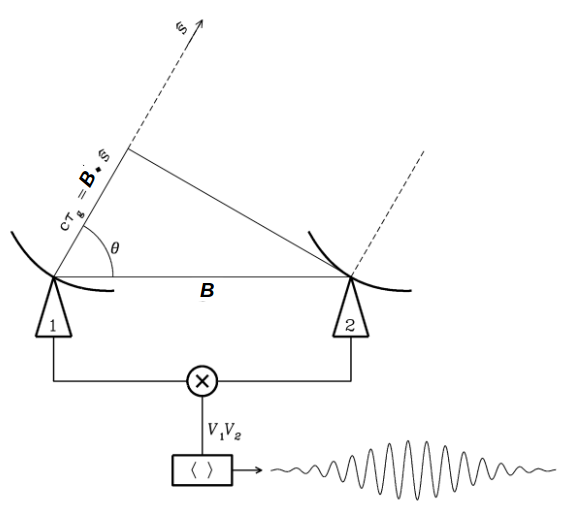
\includegraphics[scale = 0.5]{interferometer_edit.png}
\caption{A two element interferometer observing an arbitrary source in the direction $\widehat{\textbf{\textit{s}}}$, with the baseline \textbf{\textit{B}}. The two elements are represented as 1 and 2 with V$_1$ and V$_2$ as their respective visibilities. `X' represents the correlator where the multiplication and averaging of the signal takes place.}
\label{interf}
\end{figure}
\begin{equation}
<\textrm{V}_1 \textrm{ V}_2 > = \frac{\textrm{V}^2}{2}\textrm{cos} \left( \frac{\omega_c \vert  \textbf{\textit{B}} \vert }{c} \textrm{sin} \theta \right) 
\end{equation}
\noindent The correlator response is dependent sinusoidally on the direction of the source. This implies that there may be a loss of data at some values of $\theta$. Hence, a second correlation is done between outputs of the antennae with a $\pi$/2 phase delay on one of the outputs.
\subsection{UVW coordinate system}
The UVW system is used in radio interferometry due to its feasibility of use. It is expressed with a reference direction of `phase center' which remains fixed to the sky, and is often in the same direction of the delay centre\footnote{
\begin{alignat}{2}
  &&\textrm{Fringe washing function} 
  &= sinc(\pi \tau_g \bigtriangleup \nu) 
  = \frac{\textrm{sin} (\pi \tau_g \bigtriangleup \nu)}{\pi \tau_g \bigtriangleup \nu}\\
  &\Rightarrow\quad
  &<\textrm{V}_1 \textrm{ V}_2 > &= \frac{\textrm{V}^2}{2}\textrm{cos}(\omega_c \tau_g) \textrm{sinc}(\pi \tau_g \bigtriangleup \nu)
\end{alignat} It diminishes the interferometer response. Thus, one may choose the direction in which the Fringe washing function is zero, called the \textbf{delay center}.}. This system is a right handed Cartesian coordinate system. U and V are on a plane perpendicular to the phase centre with U in the East West direction and V in the North South direction, as can be seen in the  Figure  \ref{UVcomp}. W is in the direction of the phase center. Usually, the coordinates are expressed in terms of the wavelength of the observation.
\begin{center}
(u,v,w) = $\frac{\textbf{\textit{B}}}{\lambda}$ = $\vec{\textrm{B}}_\lambda$
\end{center}
The UV visibilites are obtained consecutively in time, which makes the baseline vector to rotate in the UVW plane. Thus, the UV coverage is the set of uv values for which the visibilities are obtained. LOFAR visibilities are stored in MeasurementSet format, in which the (u,v,w) data is stored in meters, thus preventing the confusion between various frequency channels in the observation.
\begin{figure}[h]
    \centering
    \subfloat[]{{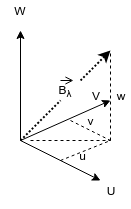
\includegraphics[scale=0.6]{UVW.png} }%
    \label{UV1}}
    \qquad
    \subfloat[]{{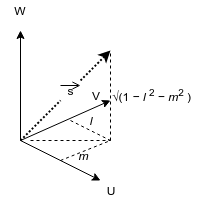
\includegraphics[width=4.5cm]{LM.png} }
    \label{UV2}}%
    %\qquad
    \subfloat[]{{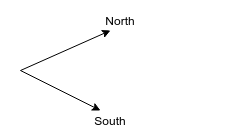
\includegraphics[width=4.5cm]{NE.png} }
    \label{UV3}}
    \caption{The UVW coordinate system. \textit{Left}: The (u,v,w) coordinates, along with the directions. The $\vec{\textrm{B}}_\lambda$ represents the direction of the source in UVW coordinate system. \textit{Middle}: The (l,m) coordinate system on the image plane, which is visited upon again section A.1. \textit{Right}: The Earth EWNS directions.}
\label{UVcomp}
\end{figure}
\subsection{Calibration techniques used for LOFAR calibration}
LOFAR calibration used the RIME formalism, which is explained in detail in the Appendix. With the help of the Van Zitter Zernike theorem, the true visibilities for an image can be obtained. While this may seem simple enough, there are several challenges that come with synthesis of an image. The true visibility is corrupted by antenna based effects such as atmospheric attenuation, variable pointing offsets, variable delay offsets, electronic gain, delay and phase changes. It may also be corrupted by baseline based effects such as radiometer noise, correlator malfunctions and RFI. Some of the methods to circumvent the problems are discussed below:
\paragraph{Convolutional gridding:}
To synthesise an image from the UV data, one first has to transform the non-uniformly sampled UV-plane into a uniformly sampled UV plane. This is done with the help of convolutional gridding. The data is first convolved with a appropriate function (such as a SHAH function) so that a uniform UV grid can be generated. This is followed by the IFFT an element by element division is done on the image plane intensity. This generates the `dirty image', which is then deconvolved to give a clean image. 
\paragraph{W-projection:}
In case of a small field of view, the w-term can be neglected. However, this cannot be done in the case of LOFAR. One of the methods to take care of this term is the w-projection algorithm, in which a visibility sample is projected onto a w=0 plane so the effects of the term get nullified. This is followed by the convolutional gridding to obtain the image \citep{2008ISTSP...2..647C}. Another algorithm is the w-stacking algorithm in which the correction is applied after the visibilities are gridded \citep{2012SPIE.8500E..0LC}.
\paragraph{Direction dependent calibration:} 
In LOFAR, the field of view is very large. This proves to severely affect the image of sources that are not point-like, for example, a galaxy like IC\,342. This is because the total electron content is different for LOFAR in every direction in its field of view. As can be seen in the Figure \ref{fovl}, the variation of the TEC is explained for different array configurations.

\begin{figure}[h]
\centering
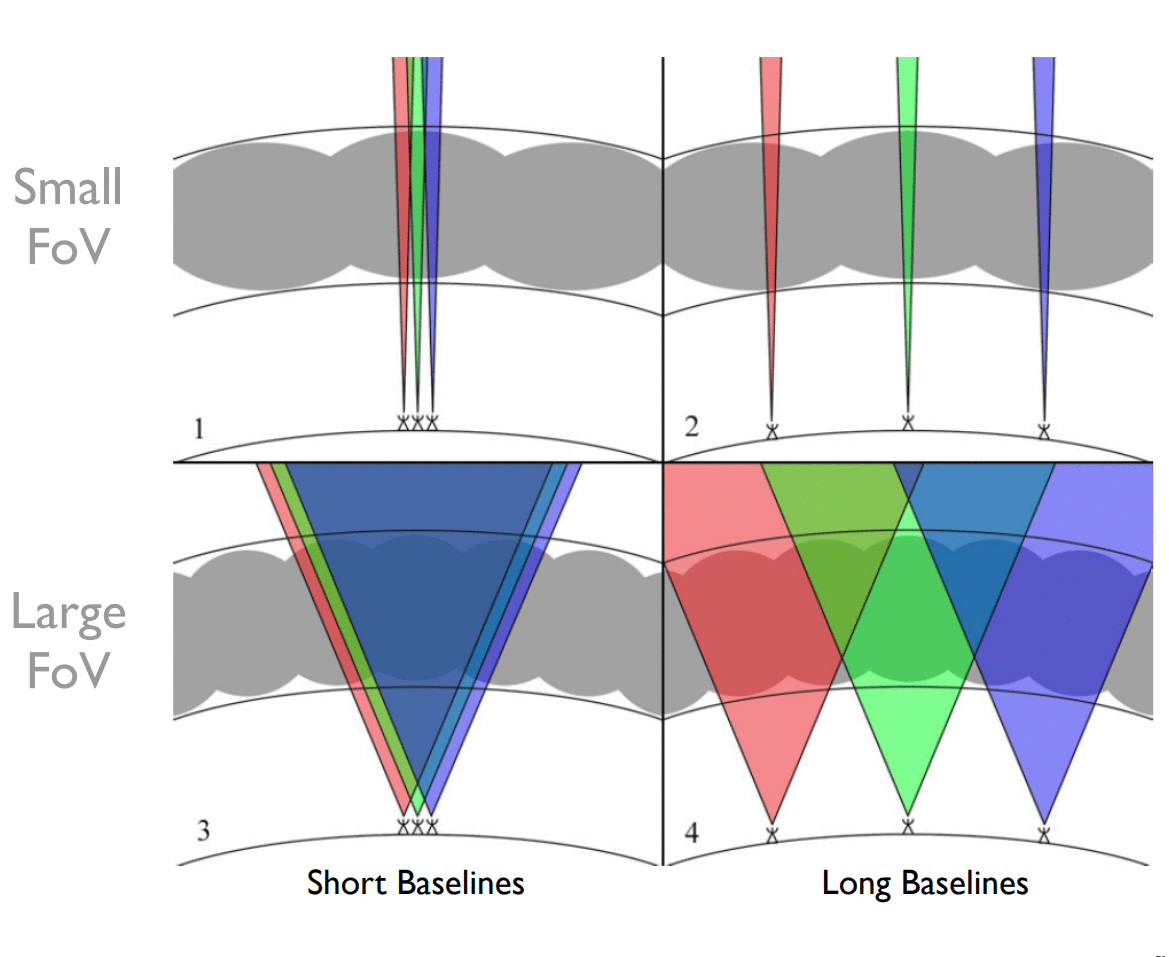
\includegraphics[scale = 0.28]{loffov.png}
\caption{LOFAR is represented by three antennas at ground level. The ionospheric electron density structure (grey bubbles)are shown, with the various fields of view shown in (red, green and blue areas). For antennae like VLA, the primary beam patterns, shown in regimes 1 and 2, each individual antenna has the field of view in which the TEC stays approximately the same. The primary beam patterns in LOFAR are more like the ones shown in regimes 3 and 4. The TEC along the line of sight in the field of view has variations. In regimes 1 and 3, the relatively compact array configurations are shown. The TEC variation across the array for a single viewing direction within the FoV is approximately a gradient. In regimes 2 and 4, relatively extended array configurations are shown. The TEC variation varied significantly for the fields of view in such configurations. This image has been taken from \citet{2009A&A...501.1185I}, where a very good description of the calibration techniques is given.}
\label{fovl}
\end{figure}

In order to obtain better images, LOFAR calibration uses a method called faceting, in which the field of view is divided into smaller fields containing a strong source or a small group of sources with a high flux density. Some of the higher flux density objects have enough Signal-to-Noise (S/N) to calibrate themselves, to obtain a better image. Thus, self-calibration is performed using these strong sources. Using the method of self-calibration, the sensitivity of the image can be greatly improved. Sometimes, the increase in effective S/N may even be an order of magnitude better. Hence, a better gain calibration can be done with just an approximate source image, to give a much better final image of the source. 


\subsection{Overview of imaging procedure for LOFAR}
\label{sec:sky_model}
In this section, a brief overview of how the data from the CEP cluster is imaged is given. The pipeline and the procedure I have used my differ slightly from the procedure given in this section. \\
\noindent The data from the CEP clusters is in the form of measurement sets. This data undergoes \textbf{pre-processing}. In this stage, the data is flagged in both time and frequency domains (even averaging of data may be done in both domains at this stage, if need be). After this, demixing is done. This is the subtraction of the brightest sources in the low frequency sky (the A-team\footnote{Cassiopeia A, Cygnus A, Taurus A, Virgo A, Hydra A, and Hera A}). A round of initial calibration is applied, which is done using a standard flux calibrator reference source. Then an initial phase calibration is performed. The Local Sky Model (LSM) used for this is obtained from the Global Sky Model (GSM). This uses 4 major catalogues: VLA Low--frequency Sky Survey (VLSS) \citep{vlss2}, Westerbork Northern Sky Survey (WENSS) \citep{wenss}, the NRAO VLA Sky Survey and (NVSS) \citep{nvss} and the Multifrequency Snapshot Sky Survey (MSSS) \citep{msss}. For removing any remaining RFI/ noise, another round of flagging and filtering is done. \\
After the pre-processing of the data, the \textbf{imaging} procedure is started. The non-coplanarity effects (the \textit{\textbf{w}} term of the equation \ref{wterm}) are removed using an algorithm, especially when doing wide field imaging. This is followed by taking care of the antenna primary beam variations which depend on the time, frequency and polarization. After this, a source finding algorithm is used to generate an updated LSM. Finally, a final round of flagging, imaging and LSM model updating is done. The final image products are then made available in the LTA.\\
\end{document}
